\documentclass{article}
\author{NAME}
\title{TITLE}
\usepackage{enumerate}
\usepackage{fancyhdr}

\usepackage{enumerate}
\usepackage{tikz}
\usetikzlibrary{automata,positioning}

% see http://nlp.stanford.edu/manning/tex/ for full documentation

\pagestyle{fancy}
\lhead{\today}
\chead{TITLE}
\rhead{NAME}

\begin{document}
	\begin{enumerate}[(a)]
		\item
		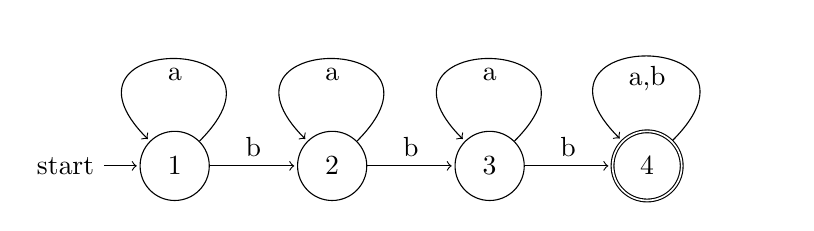
\begin{tikzpicture}[shorten >=1pt,node distance=2cm,on grid,auto] 
		\node[state,initial] (1)   {$1$}; 
		\node[state] (2) [right=of 1]{$2$};
		\node[state] (3) [right=of 2]{$3$};
		\node[state,accepting] (4) [right=of 3]{$4$};
		\path[->] 
		(1) edge  node {b} (2)
		edge [loop] node {a} ()
		(2) edge node {b} (3)
		edge [loop] node {a} ()
		(3) edge node {b} (4)
		edge [loop] node {a} ()
		(4) edge [loop] node {a,b} ();
		\end{tikzpicture}
		\item
		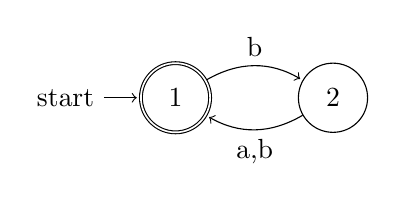
\begin{tikzpicture}[shorten >=1pt,node distance=2cm,on grid,auto] 
		\node[state,initial,accepting] (1)   {$1$}; 
		\node[state] (2) [right=of 1]{$2$};
		\path[->] 
		(1) edge [bend left] node {b} (2)
		(2) edge [bend left] node {a,b} (1);
		\end{tikzpicture}
		\item
		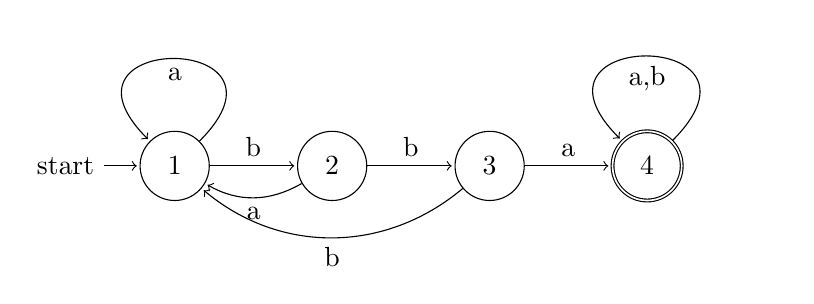
\begin{tikzpicture}[shorten >=1pt,node distance=2cm,on grid,auto] 
		\node[state,initial] (1)   {$1$}; 
		\node[state] (2) [right=of 1]{$2$};
		\node[state] (3) [right=of 2]{$3$};
		\node[state,accepting] (4) [right=of 3]{$4$};
		\path[->] 
		(1) edge  node {b} (2)
		edge [loop] node {a} ()
		(2) edge node {b} (3)
		edge [bend left] node {a} (1)
		(3) edge node {a} (4)
		edge [bend left=40] node {b} (1)
		(4) edge [loop] node {a,b} ();
		\end{tikzpicture}
		\item
		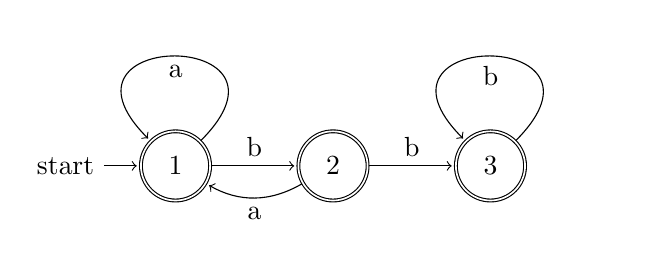
\begin{tikzpicture}[shorten >=1pt,node distance=2cm,on grid,auto] 
		\node[state,initial,accepting] (1)   {$1$}; 
		\node[state,accepting] (2) [right=of 1]{$2$};
		\node[state,accepting] (3) [right=of 2]{$3$};
		\path[->] 
		(1) edge  node {b} (2)
		edge [loop] node {a} ()
		(2) edge node {b} (3)
		edge [bend left] node {a} (1)
		(3) edge [loop] node {b} ();
		\end{tikzpicture}
	\end{enumerate}
\end{document}

